%Siehe tolle Daten in Tab. \ref{tab:impl:data}.
%
%%\begin{table}
%%    \centering
%%    \begin{tabular}{|lcc|}
%%    \hline
%%              & \textbf{Regular Customers} & \textbf{Random Customers} \\ \hline
%%    Age       & 20-40                      & \textgreater{}60          \\ \hline
%%    Education & university                 & high school               \\ \hline
%%    \end{tabular}
%%    \caption{Ein paar tabellarische Daten}
%%    \label{tab:impl:data}
%%\end{table}
%%
%%\begin{figure}
%%    \centering
%%    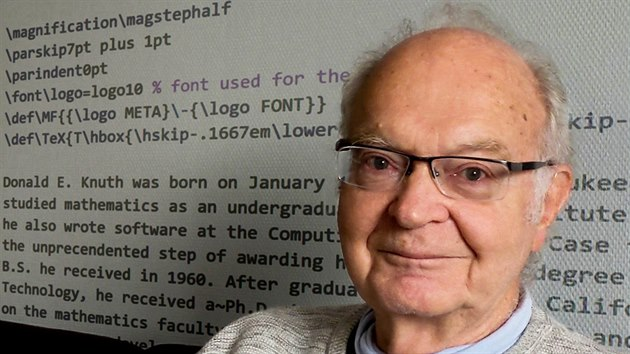
\includegraphics[scale=0.5]{pics/knuthi.jpg}
%%    \caption{Don Knuth -- CS Allfather}
%%    \label{fig:impl:knuth}
%%\end{figure}
%%
%%Siehe und staune in Abb. \ref{fig:impl:knuth}.
%%\lipsum[6-9]
%%Dann betrachte den Code in Listing \ref{lst:impl:foo}.
%%
%%\begin{lstlisting}[language=Python,caption=Some code,label=lst:impl:foo]
%%# Program to find the sum of all numbers stored in a list (the not-Pythonic-way)
%%
%%# List of numbers
%%numbers = [6, 5, 3, 8, 4, 2, 5, 4, 11]
%%
%%# variable to store the sum
%%sum = 0
%%
%%# iterate over the list
%%for val in numbers:
%%    sum = sum+val
%%
%%print("The sum is", sum)
%\end{lstlisting}

\section{Aufbau}\label{sec:assembly}

Folgend werden alle Gegenstände und Geräte für den Aufbau in Abbildung~\ref{fig:assembly} benannt.

\begin{figure}
    \centering
    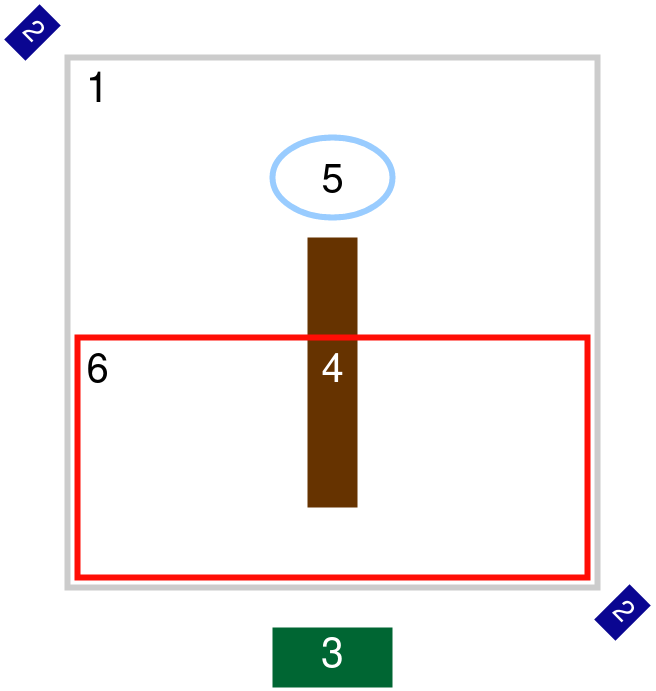
\includegraphics[scale=0.5]{pics/assemlbly}
    \caption{Aufbau}
    \label{fig:assembly}
\end{figure}

\begin{enumerate}
    \item VR Raum
    \item Lichtboxen~\ref{sec:lighthouse}
    \item Bildschirm
    \item Balken
    \item Startposition
    \item Abgrund
\end{enumerate}

\subsection{Erklärung}\label{subsec:description}

Der Spieler bei der Startposition starten und dann Richtung Abgrund dem Balken entlang balancieren.
Die Lichtboxen müssen diagonal positioniert werden wie bereits beschrieben in dem Abschnitt~\ref{sec:lighthouse}.
Der Balken sollte ca in der Mitte sein.

Leichte Versetzungen sidn nicht tragisch. Hierbei geht es nur darum, dass der Balken nicht aus dem VR Raum
rausschaut, da das Tracking dort abbricht. Die position des Bildschirmes ist nicht wichtig.
Hierbei geht es nur um das Steam VR Setup welches bereits in dem Kapitel Steam besprochen worden ist.

\section{Code}\label{sec:code}
\subsection{Ganzkörper-Tracking}\label{sec:full-body-tracking}
\subsection{Beam Calibration}\label{subsec:beam-calibration}
\subsection{Schwerkraft}\label{subsec:gravity}
\subsection{Verkehrssystem}\label{subsec:traffic-system}
In der Stadt von BeamVR ist auf den Straßen einiges los, dass wurde mithilfe eines neuem Verkehrssystems umgesetzt.
Die Straßen sind mit, f\"ur den Spieler unsichtbaren, Objekten versehen die den Verkehr regeln.

\textbf{Car Signals}
Damit die Fahrzeuge in BeamVR wissen wo und vor allem wie sie auf den Straßen navigieren k\"onnen, wurde das Car Signal System entwickelt.
Die Car Signals gibt es in zwei verschiedenen Versionen, f\"ur die linke Straßenseite wurden gr\"une und f\"ur die Rechte Seite wurden rote Signale erstellt.
Die Signale funktionieren wie Checkpoints, jedes Auto wird nachdem es initialisiert wurde, von einem zum n\"achsten fahren.
Jeder dieser Checkpoints verweist auf den nächsten, wie in einer Liste, daher weis jedes Fahrzeug wo die momentane Zielposition ist.
\ref{fig:trafficsystem_next_signal_reference}
Endpunkte sind spezielle Signale, welche auf keinen nachfolgenden Punkt mehr verweisen, erreicht ein Auto ein solchen Punkt hat es das Ziel erreicht.

An Kreuzungen befinden sich mehrere dieser Car Signals, damit die Fahrzeuge auf der richtigen Spur bleiben und die Verkehrsregeln befolgen.
Die gr\"unen Linien zeigen die m\"oglichen Routen die das Auto fahren kann, die Pfeile visualisieren in welche Richtung gefahren werden kann.
\ref{fig:trafficsystem_crossroads}



\begin{figure}
    \centering
    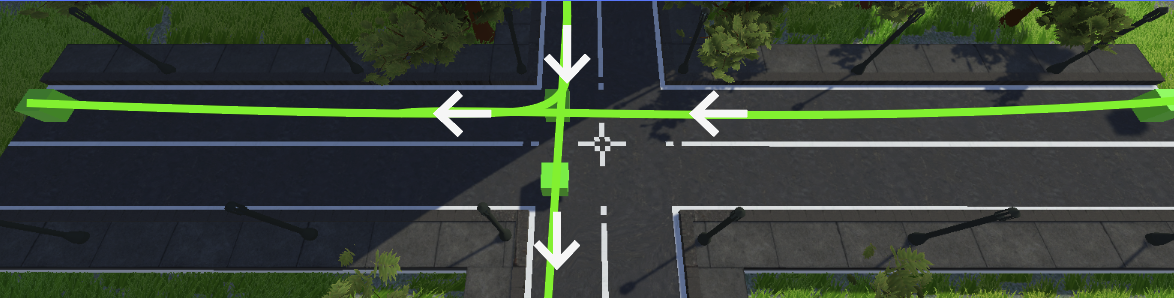
\includegraphics[scale=0.5]{pics/trafficsystem_carsignal_crossroads}
    \caption{Traffic System - Crossroads}
    \label{fig:trafficsystem_crossroads}
\end{figure}

\begin{figure}
    \centering
    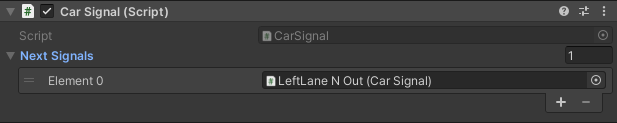
\includegraphics[scale=0.7]{pics/trafficsystem_carsignal_signal_reference}
    \caption{Traffic System - Next Signal Reference}
    \label{fig:trafficsystem_next_signal_reference}
\end{figure}


\textbf{Car Spawn Points}
Car Spawn Points sind blau dargestellte Punkte an denen Fahrzeuge, nach dem laden der Szene, initialisiert werden.
\ref{fig:trafficsystem_car_spawn_points}
Falls ein Auto einen Car Signal, welcher ein Endpunkt ist, erreicht wird es, nach einem kurzen Delay, an einem Respawn Point wieder erscheinen.
Diese Punkte verweisen, \"ahnlich wie Car Signals, auf einen nachfolgenden Punkt, wo die Fahrzeuge hinfahren.

%% IN QUELLCODEVERZEICHNIS PACKEN!
\begin{lstlisting}{CarSpawnPoint.cs}
public class CarSpawnPoint : MonoBehaviour
{

    //Location where the car should go after respawning
    public CarSignal nextSignal;

    //Position of the Respawnpoint;
    public Vector3 position;

    public void Start(){
        position = transform.position;
    }

    public Vector3 GetPosition(){
        return position;
    }

    public CarSignal GetNextSignal(){
        return nextSignal;
    }

}
\end{lstlisting}

\begin{figure}
    \centering
    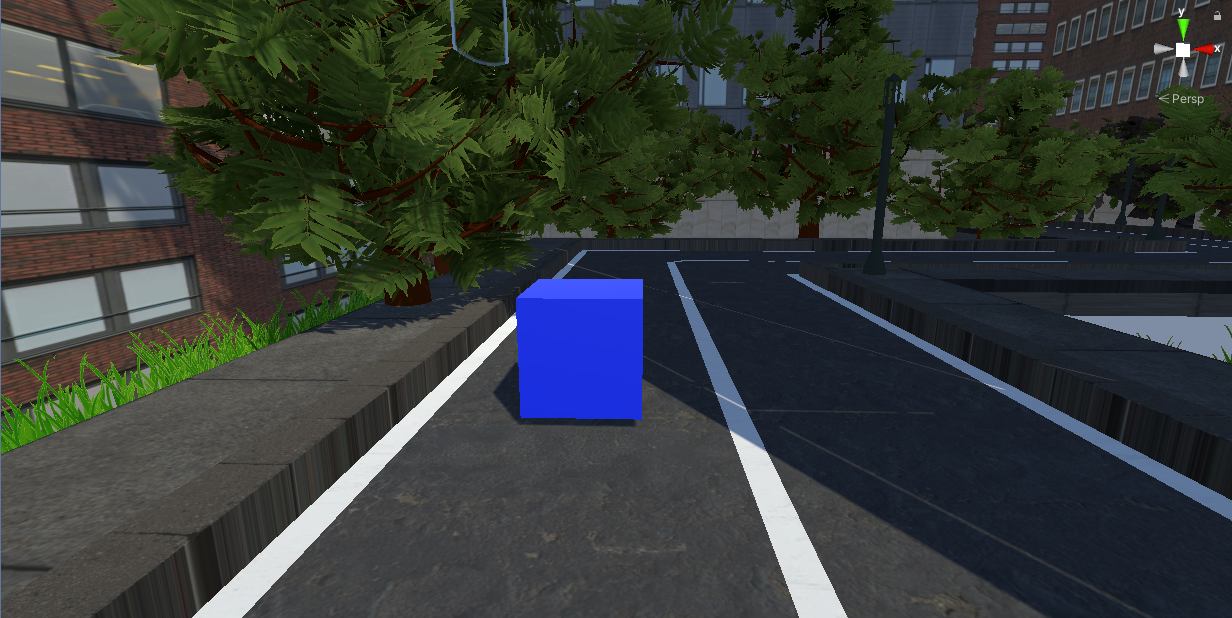
\includegraphics[scale=0.4]{pics/trafficsystem_respawn_point}
    \caption{Traffic System - Car Spawn Points}
    \label{fig:trafficsystem_car_spawn_points}
\end{figure}


\textbf{Car Manager}
Der Car Manager regelt die maximale Anzahl an Fahrzeugen die gleichzeitig auf den Straßen fahren k\"onnen.
Am Anfang werden n Fahrzeuge (n ist hierbei die maximale Anzahl an Autos) auf den Straßen initialisiert, indem ein zuf\"alliger Spawn Point ausgewählt wird.
\begin{lstlisting}{car_manager_respawncars}

public void SpawnCar(){
        CarSpawnPoint newCarSpawnPoint = GetRandomSpawnPoint();
        GameObject newCar = Instantiate(GetRandomCarModell(), newCarSpawnPoint.GetPosition(), newCarSpawnPoint.transform.rotation);
        newCar.GetComponent<CarBehaviour>().SetCarManager(this);
        CarBehaviour carBehaviour = newCar.GetComponent<CarBehaviour>();


        carBehaviour.curSignal = newCarSpawnPoint.GetNextSignal();
        carBehaviour.curPosition = newCarSpawnPoint.GetPosition();

        currentCars.Add(newCar);
    }
\end{lstlisting}

Weiters wird mithilfe der Funktion RespawnCars() ein Auto recycled, sobald es einen Endpunkt erreicht hat, indem der Manager die aktuelle Position und das n\"achste Ziel des Fahrzeuges neu setzt.
\begin{lstlisting}{car_manager_respawncars}
public void RespawnCars(GameObject finishedCar){
        CarBehaviour carBehaviour = finishedCar.GetComponent<CarBehaviour>();
        CarSpawnPoint newCarSpawnPoint = GetRandomSpawnPoint();
        carBehaviour.curSignal = newCarSpawnPoint.GetNextSignal();
        carBehaviour.curPosition = newCarSpawnPoint.GetPosition();
    }
\end{lstlisting}

\textbf{Car Behaviour}
Jedes Fahrzeug erh\"alt nachdem es initialisiert wurde eine zufällige ID mit folgendem Aufbau "Car[0-9]BeamVR[0-9]", damit diese im sp\"ateren Verlauf des Spieles besser identifiziert werden können.
In jedem Frame bewegt sich das Auto, mithilfe der Vector3.MoveTowards() Funktion, richtung dem Car signal, welches derzeit als Ziel festgelegt wurde.
Wenn nun das momentante Ziel erreicht wurde, sucht das Gefährt in dem aktuellen Punkt die Referenz auf das nächste Signal und bewegt sich dort hin.

Um zu verhindern, dass mehrere Fahrzeuge ineinander fahren,kann das Auto mithilfe eines Raycasts erkennen, was sich in einer bestimmten Distance vor sich befindet und im Notfall anhalten.

\begin{lstlisting}{car_behaviour_raycast}
...
RaycastHit hit;
         if (!Physics.Raycast(curPosition, transform.TransformDirection(Vector3.forward), out hit, carSeeingDist, layerMask))
        {
        ...
        }
...
\end{lstlisting}

\section{3d Welt}\label{sec:3d-world}
Jedes Spiel besitzt eine Spielwelt.
Babei ist es egal ob es sich um eine 3D oder 2D Applikation handelt.
Unter den Begriff Spielwelt fällt die Umgebung in welcher sich der Spieler befindet.
Es gibt hierbei so gut wie keine Einschränkungen in Bezug auf Kreativität, egal ob die digitale Welt nun ein riesiger Ring, der im Weltall schwebt,
oder eine verlassene Großstadt in einer postapokalyptischen welt, siehe Abb. ~\ref{fig:3d_environment_destiny2}.
~\cite{GamesRadar_HaloRing_2022}



%% this image and the next are not working. see issue #1

\begin{figure}
    \centering
    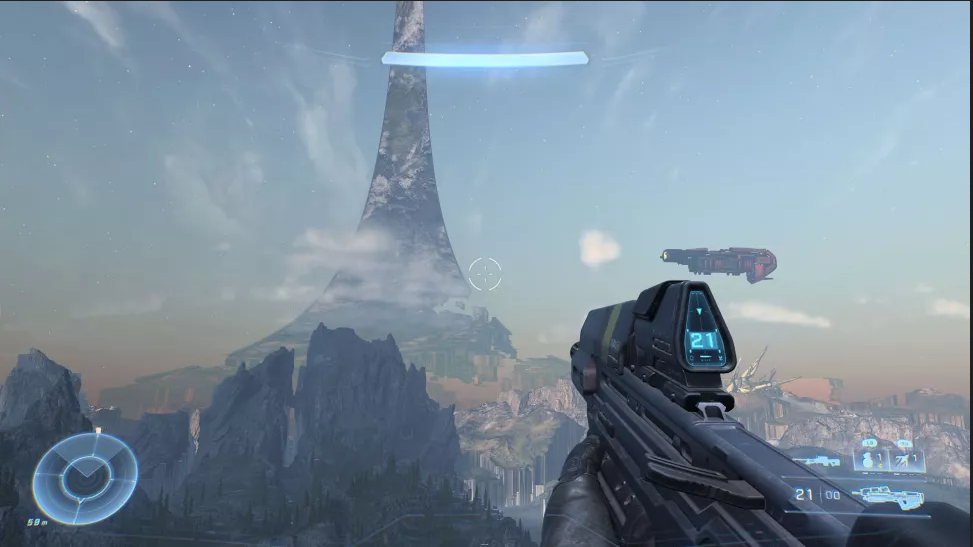
\includegraphics[scale=0.4]{pics/3d_welt_halo_ring}
    \caption{3D Welt - Halo}
    \label{fig:3d_environment_halo}
\end{figure}


%% Grafik für Destiny 2 Locations noch einbinden (Seite für Quelle lädt grade nicht Bungie.net)

\begin{figure}
    \centering
    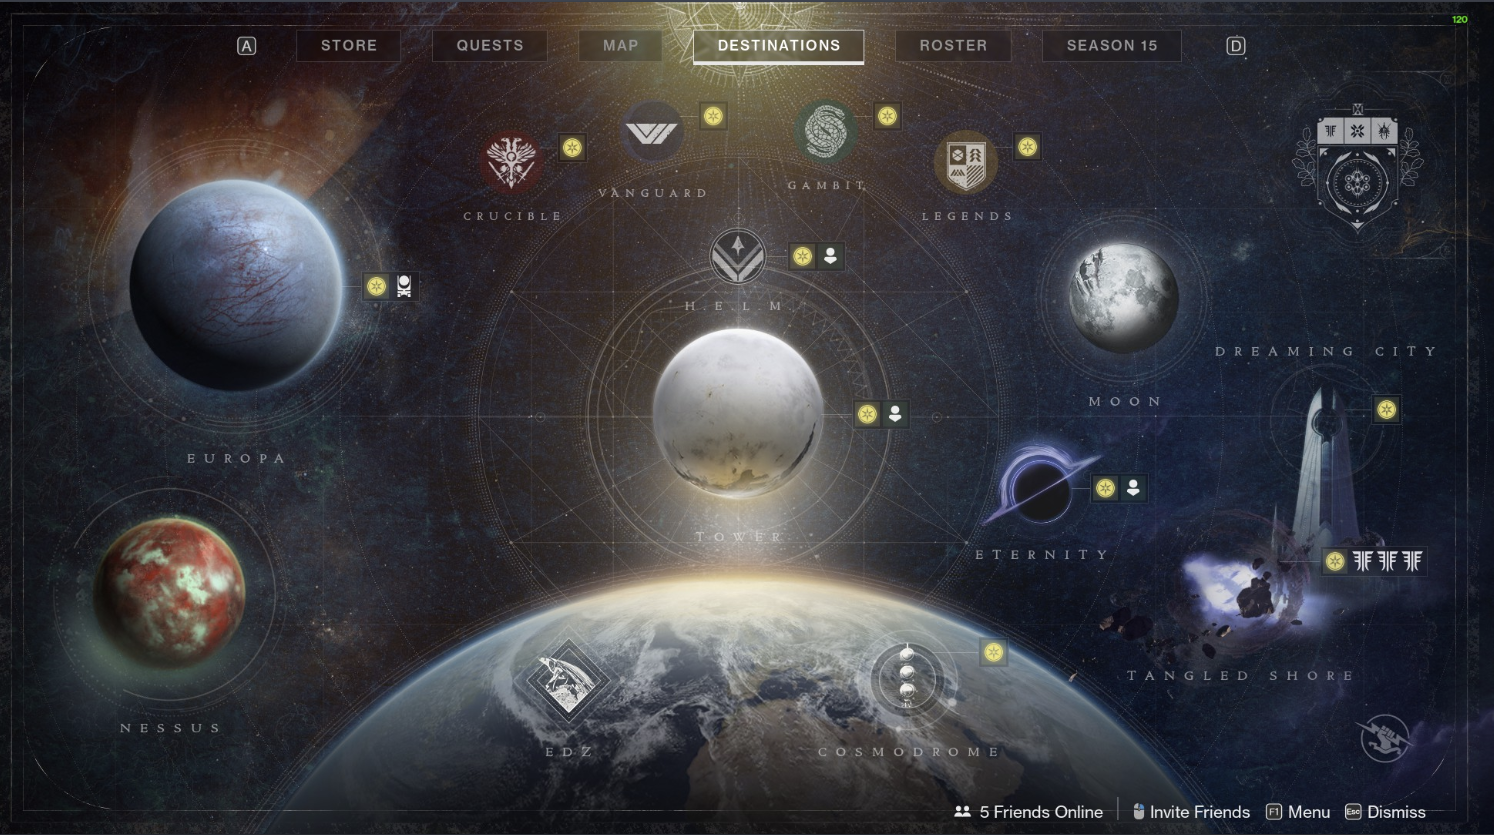
\includegraphics[scale=0.3]{pics/3d_welt_destiny_planets}
    \caption{3D Welt - Destiny 2}
    \label{fig:3d_environment_destiny2}
\end{figure}

Spielehersteller bauen die Spielwelten so auf, wie es am besten zu der Vision des Spieles passt.
Gleichzeitig wird darauf geachtet, dass sich die Umgebung nicht langweilig oder leer anfühlt.
Hierfür wird Environmental Storytelling verwendet.
Darunter versteht man das Platzieren von Gegenständen und Objekten,
welche dem Spieler eine kleine Geschichte erzählen.
Das passiert jedoch nicht über Sprache sondern einfach nur über die Platzierung und das Aussehen.
Ein Beispiel hierfür w\"are das Bild von Cayde-6 (ein Charakter aus Destiny 2), welches in einem Restaurant platziert wurde.
Cayde ist einer der drei Anführer der Vanguard, welche eine Ansammlung an Guardians (Spielern und NPC) ist und gegen das Böse kampft.
In Forsaken starb Cayde jedoch und viele trauerten um ihn, als Gedenken wurde dieses Bild aufgehangen.
~\cite{GameDeveloper_2022}

\begin {figure}
    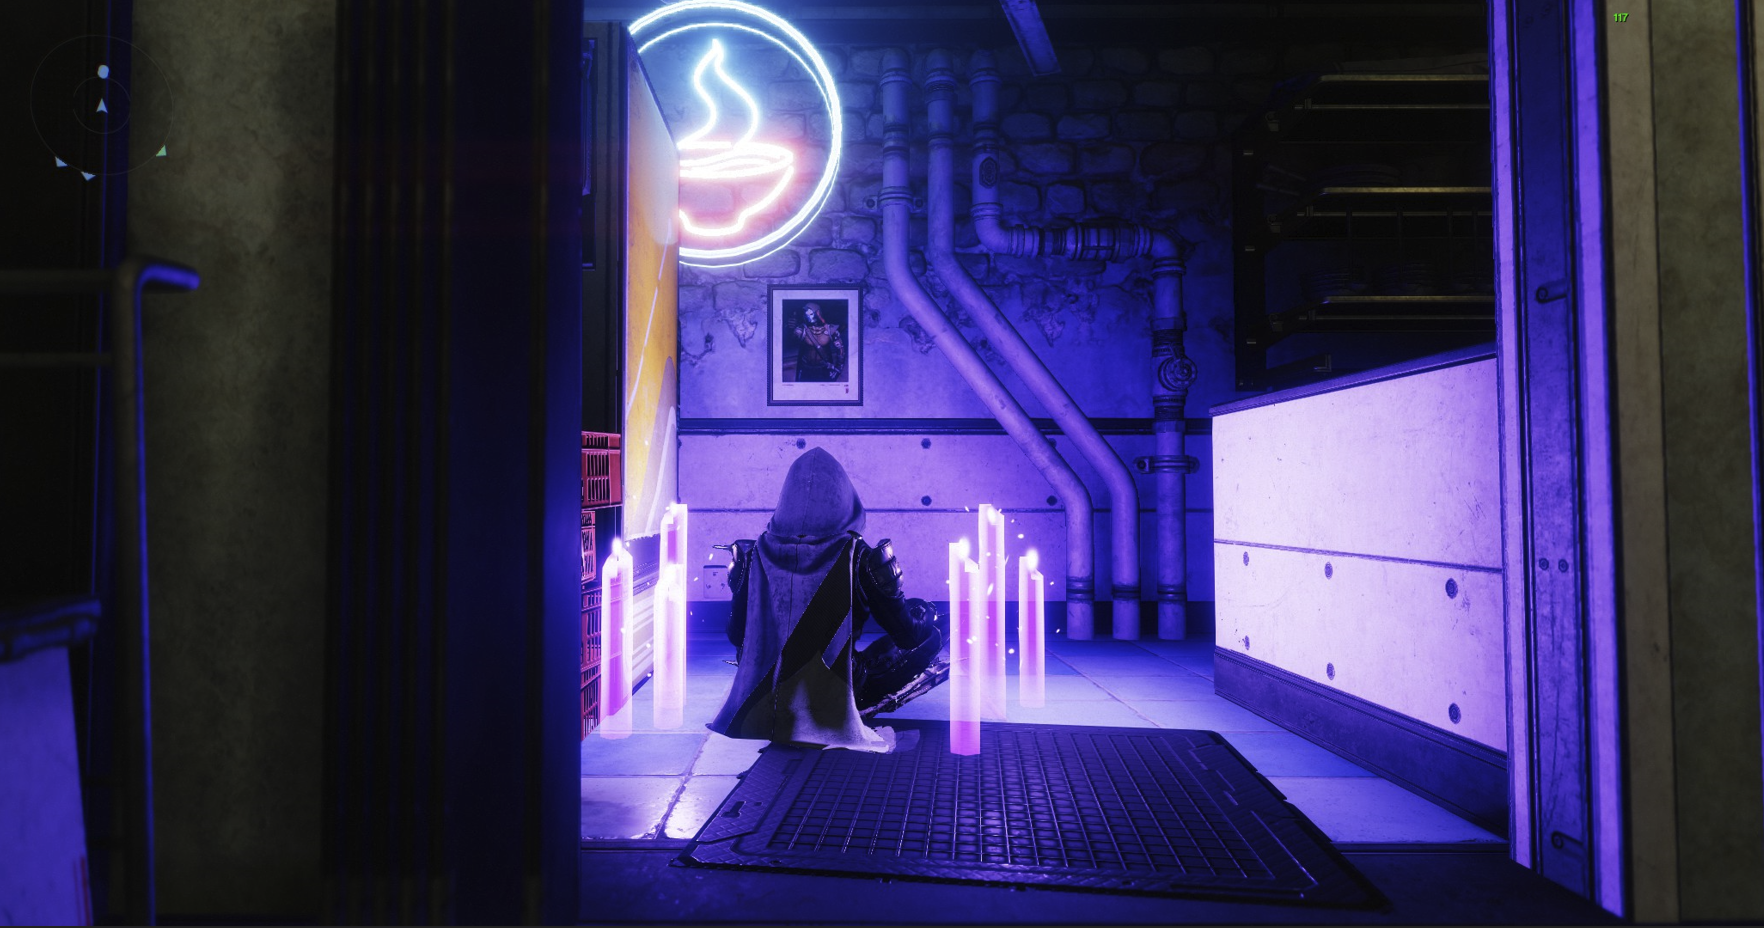
\includegraphics[scale=0.3]{pics/3d_welt_destiny2-environmental-storytelling}
    \caption{Environmental Storytelling '-' Destiny 2 Cayde}
    \label{fig:3d_environmental_storytelling_destiny2}
\end {figure}


\subsection{City Grid System}\label{subsec:city-grid-system}
Um die Gestaltung der Welt in BeamVR zu erleichtern, wurde ein Grid System verwendet.
Dafür wurde die Stadt in ein Raster aufgeteilt, an welchem sich alle Objekte der Welt auf allen 3 Achsen (x,y,z) orientieren.
~\ref{fig:grid-system-unity}
Unity stellt so ein Grid Snapping System bereits zur Verf\"ugung, daher wurde f\"ur BeamVR am Anfang der
Modellierungsphase eine Bestimmte Grid-Gr\"osse festgelegt, an dem die Grundfl\"achen der Geb\"aude und die Strassen
angepasst wurden.

\begin {figure}
    \centering
    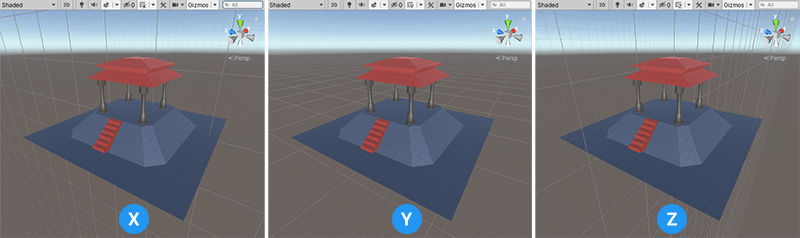
\includegraphics[scale=0.5]{pics/unity-grid-snapping}
    \caption{Unity '-' Grid Snapping System}
    \label{fig:grid-system-unity}
\end {figure}

Wenn mann die Grid Size, also die Gr\"osse des Rasters, an dem sich alles Orientiert, \"andern m\"ochte muss man zuerst das Grid and Snap Fenster aufrufen.
Als n\"achstes findet man unter dem Bereich World Grid ein Attribut namens Size, wo man die X, Y und Z Achsen frei und unabh\"angig voneinander umskalieren kann.
Wenn man alle Achsen gleichzeitig umstellen m\"ochte, muss man nur auf das Link Icon, welches sich Links neben dem X befindet, dr\"ucken.
Nun werden alle Achsen immer die gleiche Gr\"osse haben.
~\ref{fig:grid-size-unity}
~\cite{Unity_GridSnapping_2022}

\begin {figure}
    \centering
    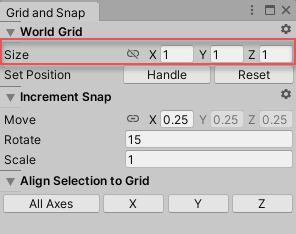
\includegraphics{pics/unity-grid-snapping-size}
    \caption{Unity - Grid Snapping Size}
    \label{fig:grid-size-unity}
\end {figure}



\subsection{Stadt}\label{subsec:city}
Jede Stadt hat viele verschiedene Strukturen wie Sehensw\"urdigkeiten, Bauwerke und Einrichtungen wie Kinos, Theater oder Restaurants.
F\"ur BeamVR wurden daher insgesamt \"uber 34 Geb\"aude Modelle erstellt um eine Vielfallt in der Umgebung zu kreieren.
~\ref{fig:beamvr_building-variety}

\begin {figure}
    \centering
    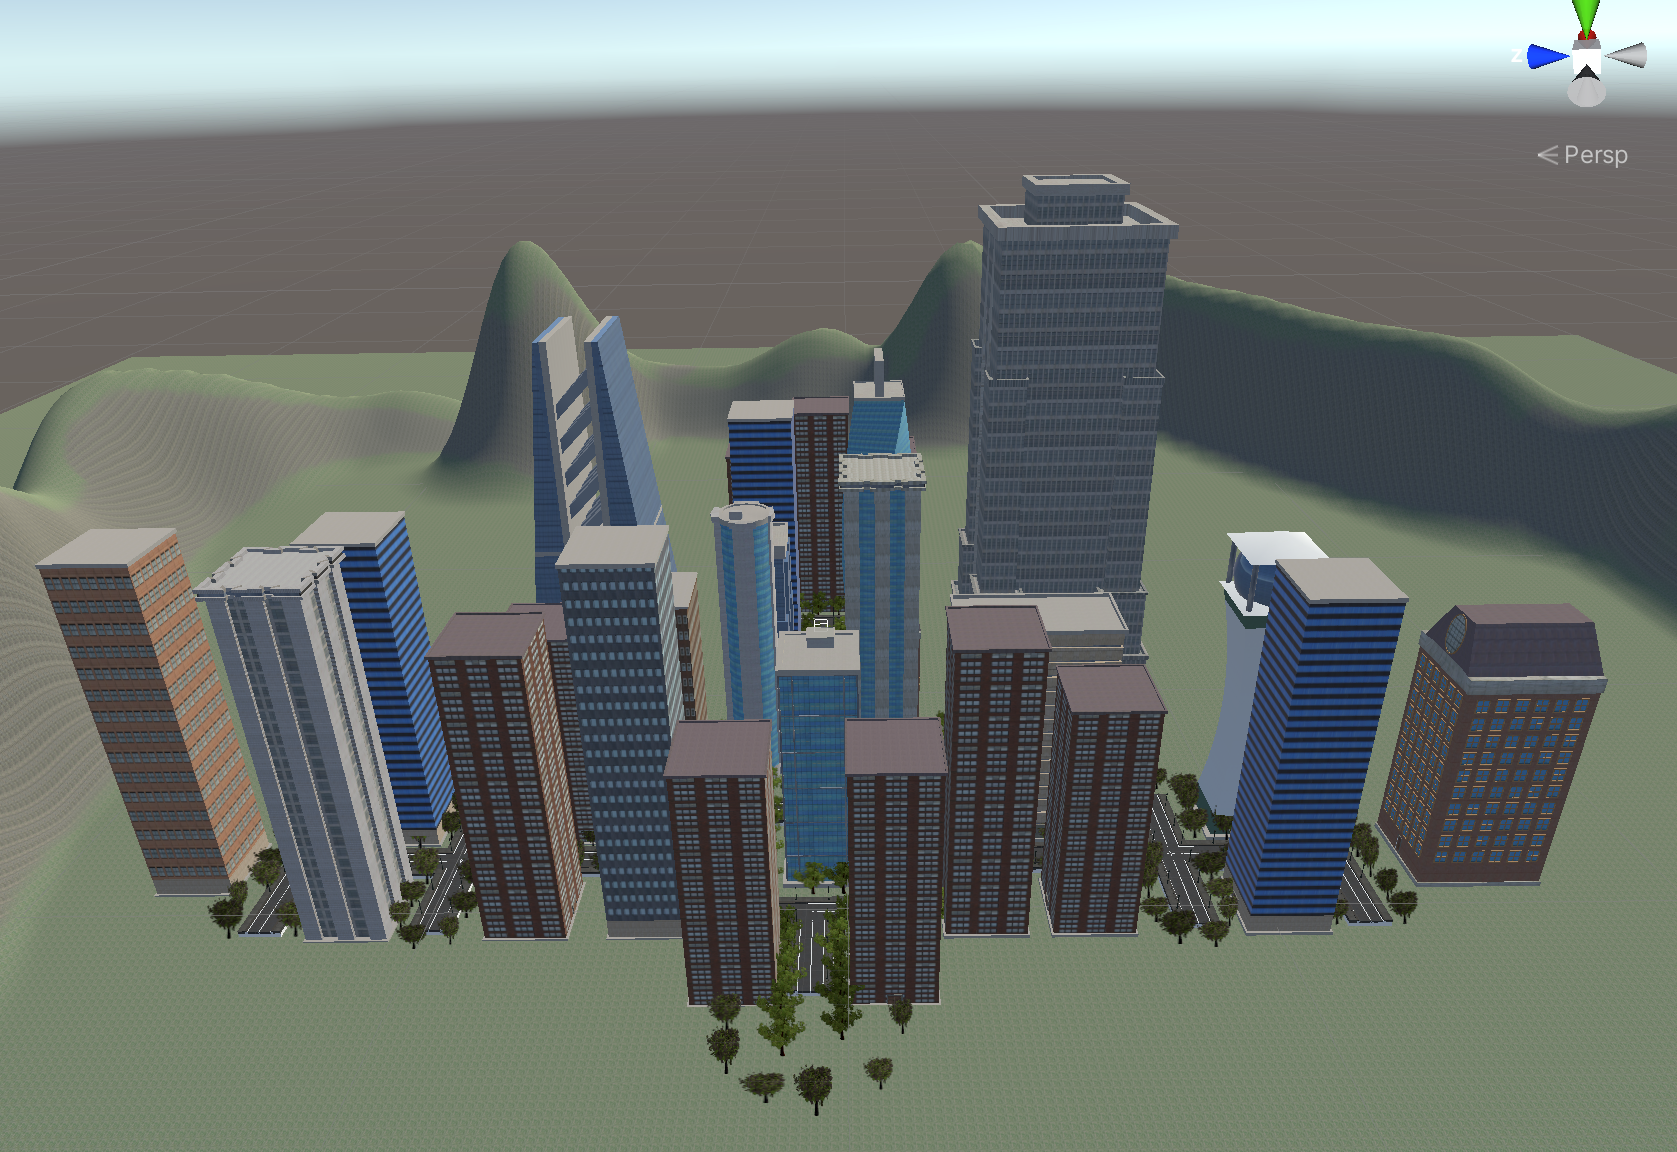
\includegraphics[scale=0.18]{pics/beamvr_building-variety}
    \caption{Beam VR - Building Overview}
    \label{fig:beamvr_building-variety}
\end {figure}

Wie auf dem Bild zu sehen, wurde die Stadt so entworfen, dass nur die für den Spieler sichtbaren Objekte wirklich existieren.
~\ref{fig:beamvr_building-variety}
Bei richtiger Umsetzung scheint es für den Anwender dennoch so, als w\"are dieser in einer kompletten Spielwelt.
In der Spieleentwicklung wird dieser Trick oft angewandt um die Performance des Spieles zu verbessern, da unn\"otige Objekte nicht gerendert oder berechnet werden m\"ussen.
Bei gr\"osseren Projekten spart das nicht nur Zeit sondern auch Ressourcen wie Geld.
Da BeamVR jedoch eine Diplomarbeit ist und daher keine Kosten w\"ahrend der Entwicklung entstehen, wurde dieser Trick angewandt
um die Frames per Second in die h\"ohe zu treiben.


\subsection{Tag Stadt}\label{subsec:day-city}
Es wurden 17 verschieden Geb\"aude f\"ur diese Map modelliert.
~\ref{fig:beamvr_building-variety}
Der Fokus bei der Gestaltung des Bauwerke lag dabei, dass diese m\"oglichst realistisch Aussehen und dennoch nicht zu Rechenaufwendig in der Darstellung werden.
Daher wurden Texturen verwendet um kleinere Details an den Fassaden darzustellen.
Das gleiche wurde bei der Apocalypsen Map angewandt.
~\ref{subsec:apocalypse-city}
Die angewandten Texturen stellen Fassaden aus Stein und Glas dar.
Ein weiterer wichtiger Punkt bei der Planung der Stadt war es auch, dass der Spieler nicht aus der Stadt raus schauen kann.
Daher wurden alle umliegenden Bauwerke mindestens 3 Meter h\"oher gemacht, als das Geb\"aude wo der Spieler steht.
~\ref{fig:beamvr_building-heights}

\begin {figure}
    \centering
    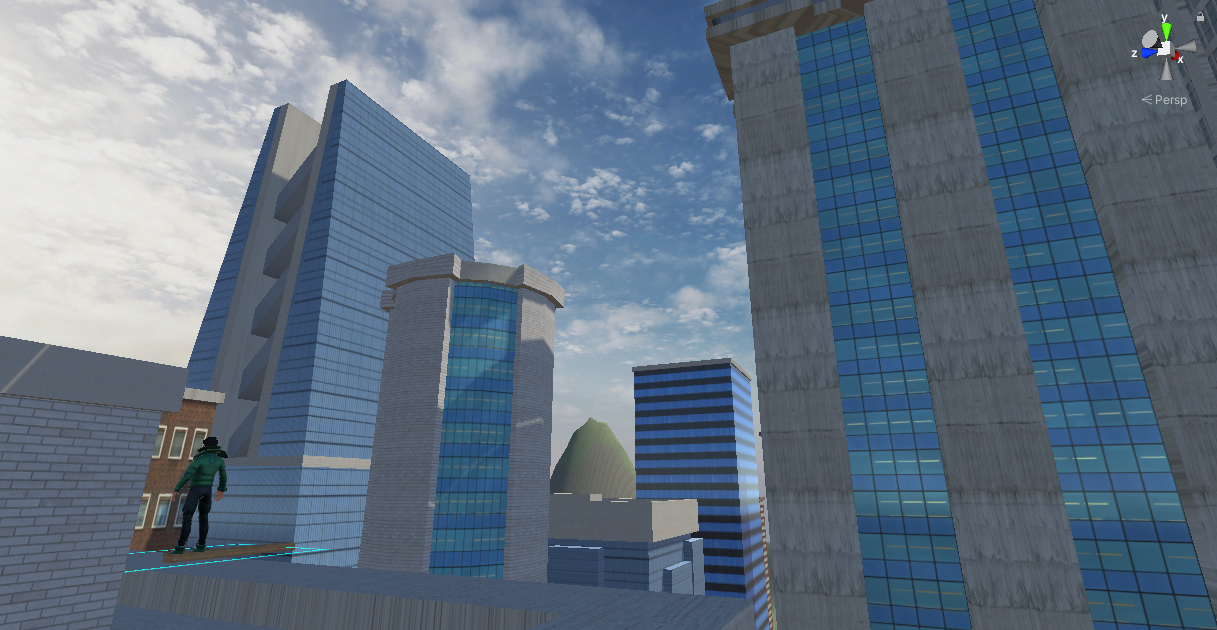
\includegraphics[scale=0.5]{pics/beamvr_city_day_heights}
    \caption{Beam VR - Building Heights}
    \label{fig:beamvr_building-heights}
\end {figure}

\subsection{Nacht Stadt}\label{subsec:night-city}
In der nacht Version der Stadt wurde die Skybox angepasst, diese zeigt nun einen Sternenhimmel.
Zus\"atzlich wurde die Belichtung der Scene auf ein bl\"auliches Licht eingestellt und die Laternen in den Straßen
haben optional noch eigene Lichtquellen.
~\ref{fig:beamvr_night_map_lighting}

\begin {figure}
    \centering
    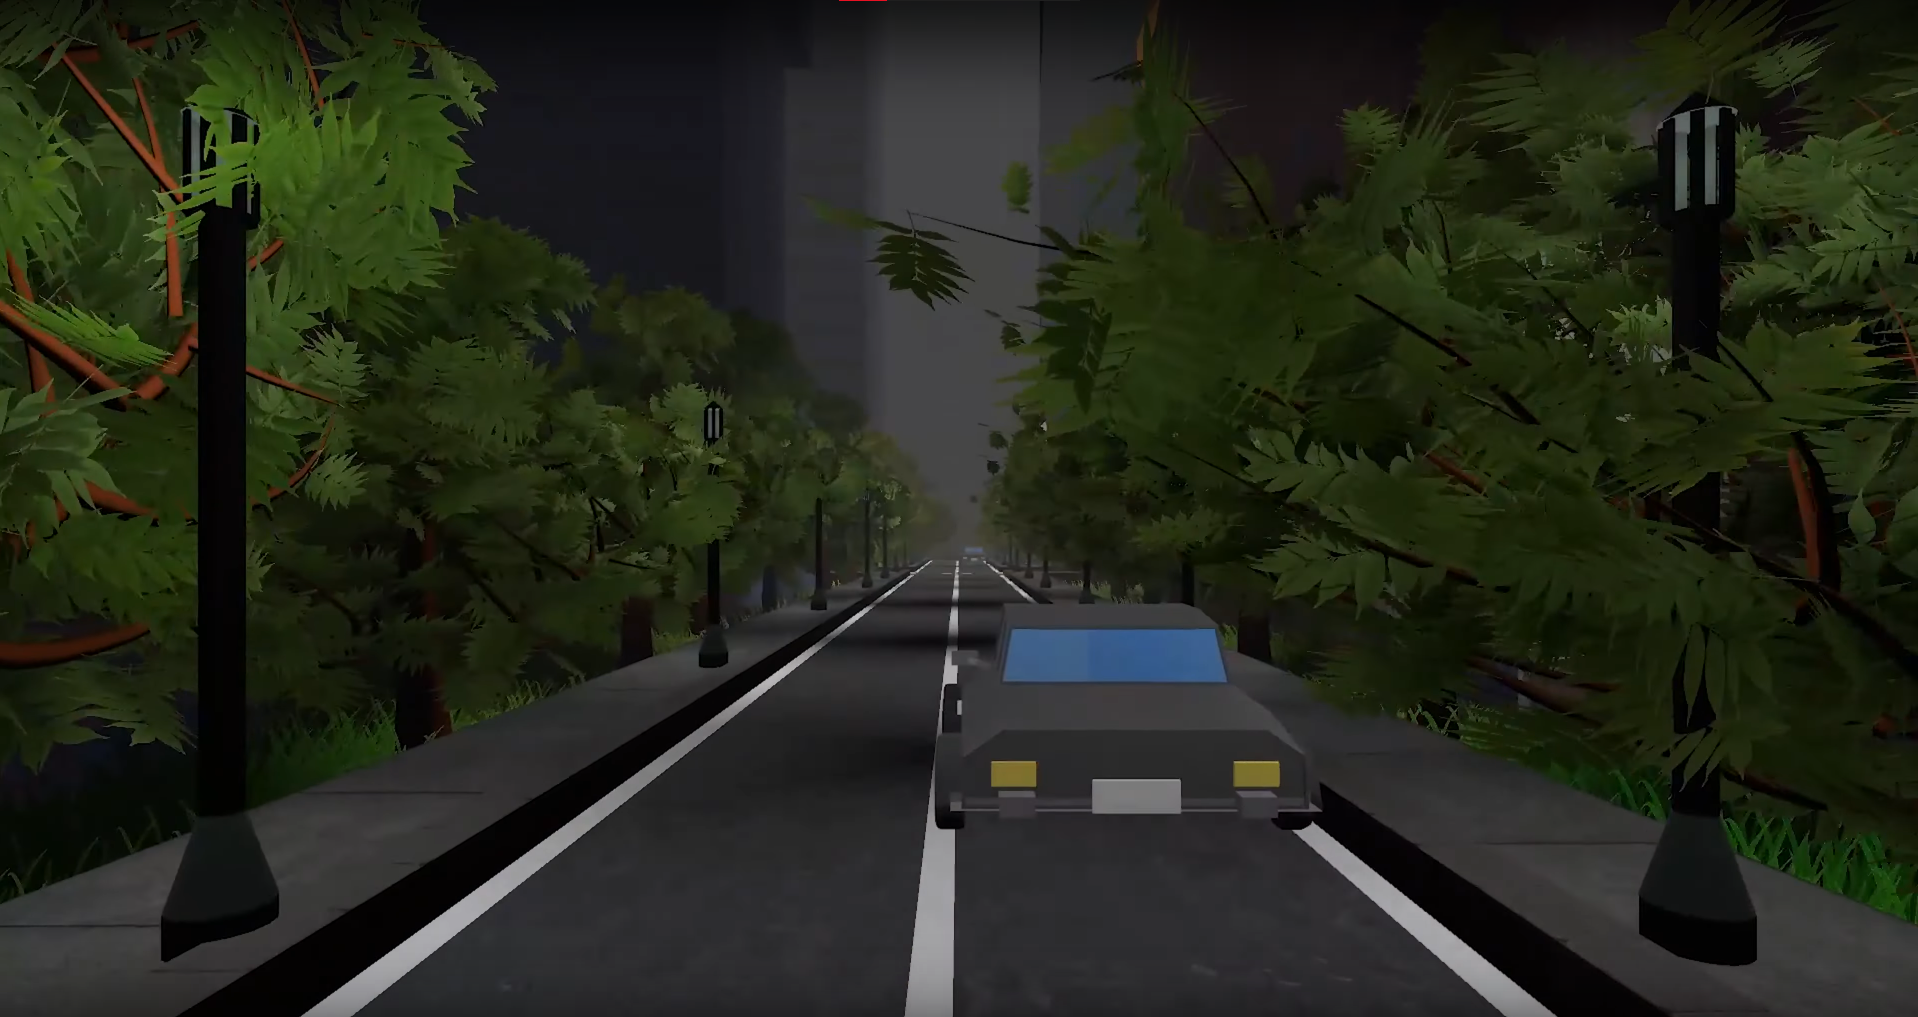
\includegraphics[scale=0.3]{pics/beamvr_night_overview}
    \caption{Beam VR - Night Map Lighting}
    \label{fig:beamvr_night_map_lighting}
\end {figure}

\subsection{Apokalypsen Stadt}\label{subsec:apocalypse-city}
F\"ur diese Umgebung wurden alle Geb\"aude nochmal \"uberarbeitet.
Statt den intakten Glasfassaden werden nun barrikadierte Fenster und Ziegelsteine ohne Verputz f\"ur die Bauwerke verwendet.
~\ref{fig:beamvr_damaged_texture}
Durch diese \"Anderung sieht die Stadt verlassen und wie nach einer Apokalypse aus.
Um den Effekt noch zus\"atzlich zu verst\"arken wurden die Bauwerke noch etwas verdreht, so dass es aussieht, als w\"urden Diese gleich umkippen.
Das Gel\"ande wurde mit neuen Sandstein Texturen und D\"unen in eine W\"uste umgewandelt.
Die Planzen und B\"aume wurden durch ausgetrocknete B\"usche ausgetauscht, damit die Welt ein trostloses aussehen bekommt.
~\ref{fig:beamvr_apocalypse_map}

\begin {figure}
    \centering
    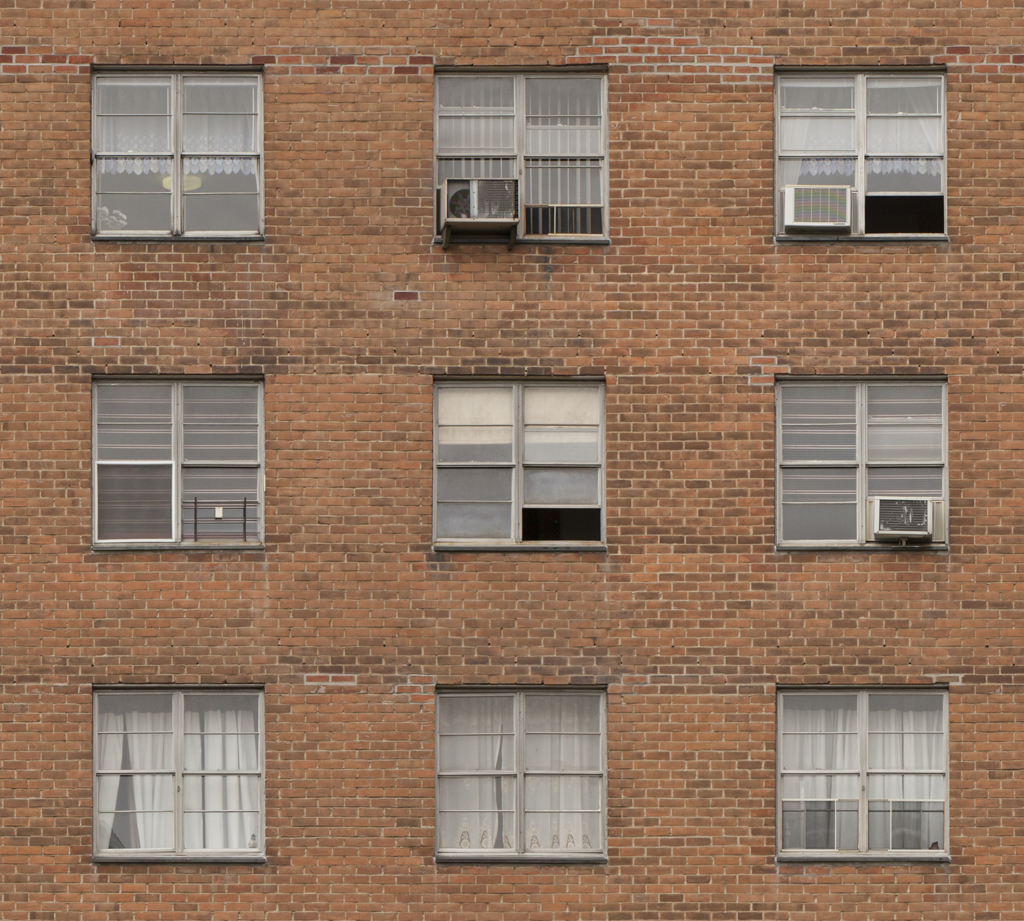
\includegraphics{pics/beamvr_damaged_texture}
    \caption{Beam VR - Damaged Texture}
    \label{fig:beamvr_damaged_texture}
\end {figure}

\begin {figure}
    \centering
    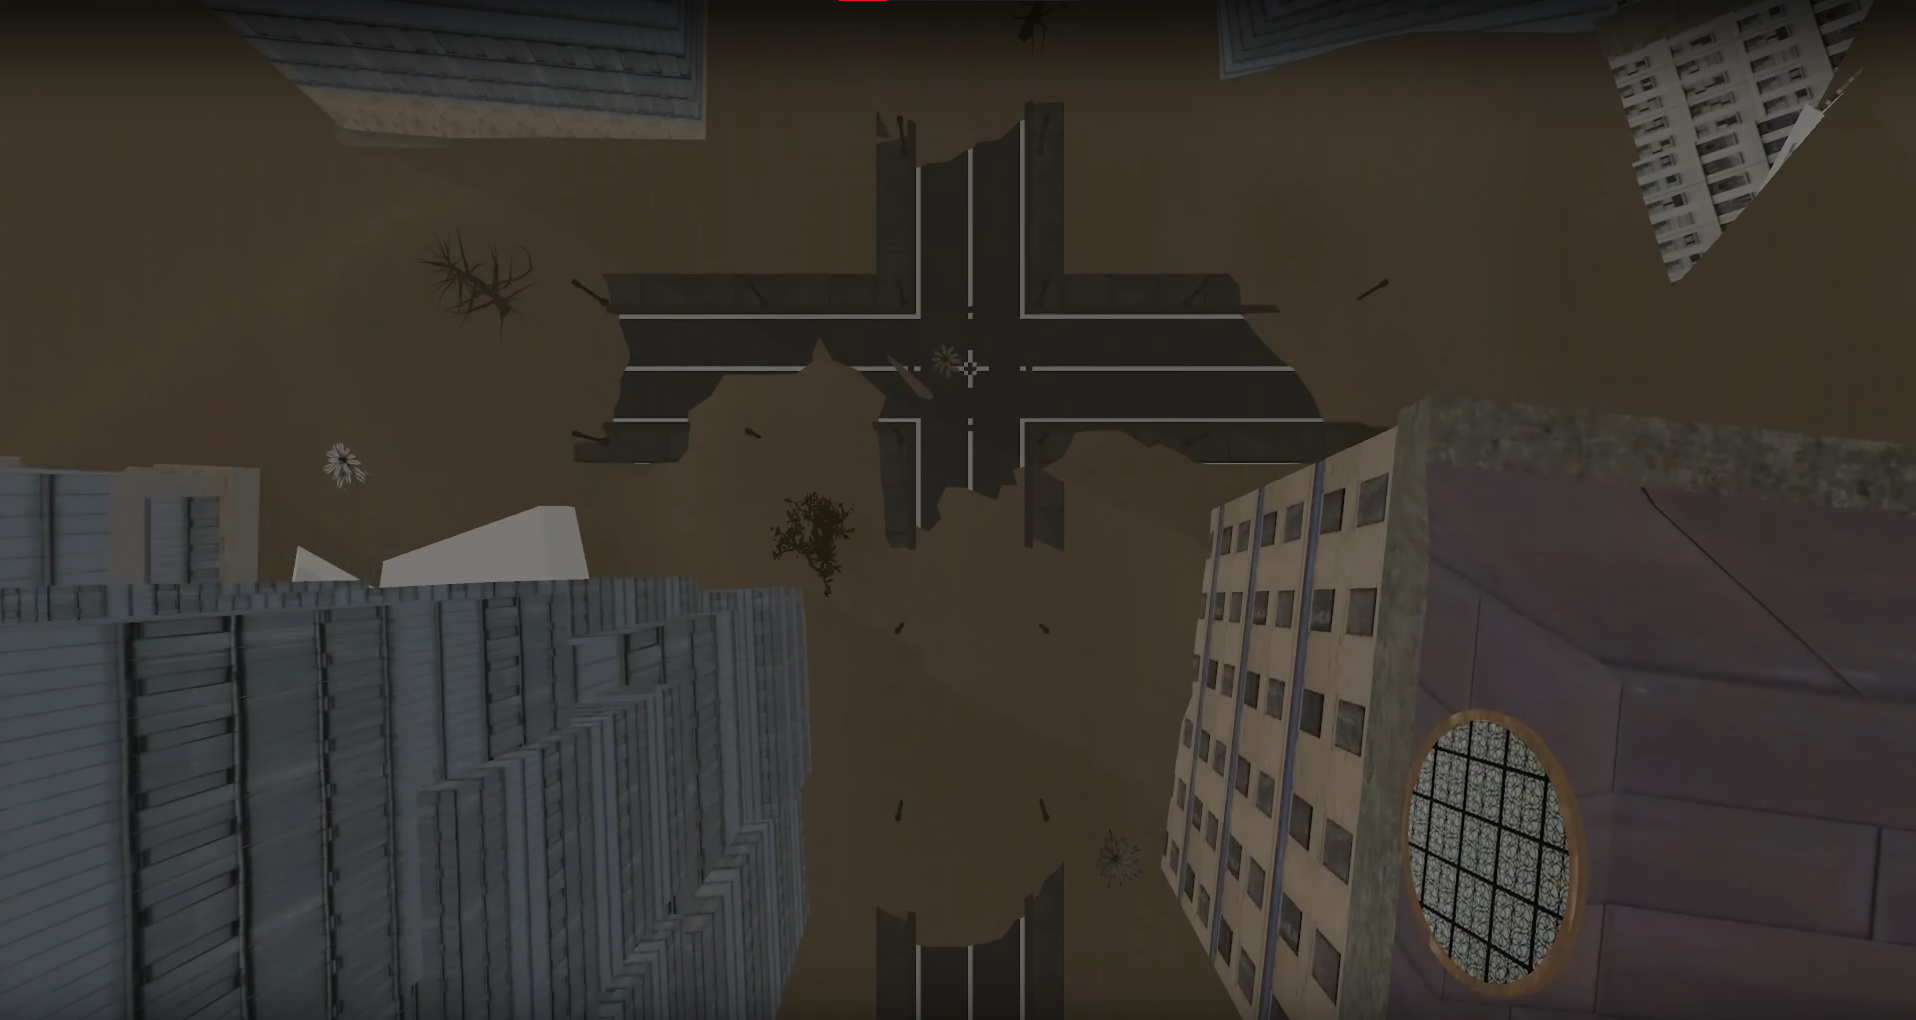
\includegraphics[scale=0.3]{pics/beamvr_apocalypse-overview}
    \caption{Beam VR - Apocalypse Map}
    \label{fig:beamvr_apocalypse_map}
\end {figure}



\section{Sound Design}\label{sec:sound}
Sound Design ist einer der wichtigsten Punkte, den man bei der Spieleentwicklung beachten muss.
In der virtuellen Umgebung der verwendeten Game Engine existieren anfangs keine Geräusche, diese m\"ussen von den Entwicklern selber erstellt und eingef\"ugt werden.


Es gibt viele verschiedene Arten Sound Design zu benutzen, wie zum Beispiel die Ger\"ausche die der Anwender selbst in der virtuellen Welt verursacht.
Wenn sich der Spieler bewegt, sollten Fußstapfen zu h\"oren sein.
Diese klingen je nach Bodentyp unterschiedlich.
Besteht der Boden aus Holz, wird man ein h\"olzernes klopfen und knarren h\"oren, ist der Boden jedoch mit Gras bedeckt wird ein rascheln abgespielt.
Zus\"atzlich wird der gesteuerte Charakter ersch\"opft klingen wenn gelaufen wurde oder gerade ein Sprung ausgef\"uhrt wird.

Bei Umgebungen ist es wichtig, dass die Welt nicht leer klingt, sondern mit situationsbedingten Hintergrundger\"auschen voller Leben erscheint.
Es gibt jedoch auch Situationen wo gezielt wenig Umgebungsger\"ausche benutzt werden um zum Beispiel eine W\"uste oder eine verlassene Stadt noch einsamer und trostloser darzustellen.

Um die Stimmung noch genauer steuern zu k\"onnen kann Musik benutzt werden.
Wenn der Spieler auf einem Pferd durch eine Weide reitet, kann eine dramatische und inspirierende Musik benutzt werden, um den Moment noch besser und cinematischer wirken zu lassen.
~\cite{GK_Media_Factory_Sound_Design_2022}

\subsection{Apocalypse}\label{subsec:apocalypse-background-sound}
Die Musik in der Apocalypse Map ist stark an das Horror Genre angelegt.
Die Melodie ist jedoch nicht wirklich existent, stattdessen existiert ein durchgehendes pfeifendes Ger\"ausch, welches unterbewusst das Spannungslevel erh\"oht.
Der Spieler f\"uhlt sich etwas unbehaglich und alleine.
Dadurch wirkt die Stadt, neben den br\"ockelnden H\"ausern, zus\"atzlich noch mehr verlassen.

Da die Sicht in dieser Map stark durch einen gelblichen Nebel, der wie ein Sandsturm wirkt, eingeschr\"ankt ist, kann man im Hintergrund den Wind pfeifen h\"oren.

\subsection{City}\label{subsec:day-night-background-sound}
Die Hintergrundger\"ausche der Tag und Nacht Version der Stadt sind sehr \"ahnlich.
Der Spieler kann Motorr\"ader und Autos auf den Straßen vorbeifahren h\"oren.
Hinundwieder kann man Menschen bei kurzen Gespr\"achen miteinander zuh\"oren und ein Kind husted im Hintergrund.

\subsection{Event}\label{subsec:building-collapse-sound}
Um spezifische Events, also bestimmte Dinge welche in der Welt passieren, f\"ur den Benutzer besser erkennbar zu machen, wurden zus\"atzlich Ge\"ausche eingef\"ugt.
Auf der Apocalypse Map sind zusammenbrechende Geb\"aude zu h\"oren, um die schlechte instandhaltung der verlassenen Stadt erneut hervorzuheben.
Aber wenn der Benutzer genauer hinsieht, kann man w\"ahrend diese Sounds h\"orbar sind, auch tats\"achlich eine kleine Auswahl an Bauwerken br\"ockeln sehen.

\section{Effects}\label{sec:effects}
Unity bietet verschiedene M\"oglichkeiten um das Aussehen der Applikation zu beeinflussen.
Mithilfe von Post Processing kann man Filter und Effekte zu dem Buffer der Kamera hinzuf\"ugen bevor etwas am Bildschirm Angezeigt wird.
Eine kleine Auswahl von diesen Effekten und Filtern sind zum Beispiel Bloom, Grain oder Color Grading.
~\cite{Unity_Post_Processing_2022}

Post Processing kann Global angewandt werden, somit werden die eingestellten Filter \"uber die komplette Spielwelt angewandt.
Um das zu erreichen muss einfach nur eine Option namens IsGlobal ausgew\"ahlt werden.
Um die Effekte auf einen bestimmten Bereich zu begrenzen muss ein Collider erstellt und platziert werden.
Wenn die Kamera in diesem Collider ist, wird das angezeigte Bild mit den eingetellten Effekten versehen.
~\cite{Unity_Post_Processing_Volumes_2022}


\subsection{Nebel}\label{subsec:fog-effect}
Unity bietet mehrere M\"oglichkeiten Nebel darzustellen, wie zum Beispiel mithilfe von Post Processing oder mithilfe der Lighting Einstellungen.
F\"ur BeamVR wurde die Lighting Variante verwendet.
Unter Settings > Lighting befindet sich eine Checkbox names Fog.
Wenn man diese Anklickt wird automatisch eine standard Einstellung f\"ur einen Nebel dargestellt.
~\cite{Unity_Fog_2022}

Auf fast jeder Map von BeamVR wurde dieser Nebel verwendet.
In der Nacht Map wird mithilfe diesem Effekts ein leichter Nebel dargestellt, was zur abendlichen Stimmung beitr\"agt.
Bei Apocalypse ist der Nebel viel dichter und stellt einen Sandsturm dar. Zus\"atzlich wurde dieser gelb gef\"arbt um noch mehr an Sand zu erinnern.
~\ref{fig:beamvr_yellow_fog}
\begin {figure}
    \centering
    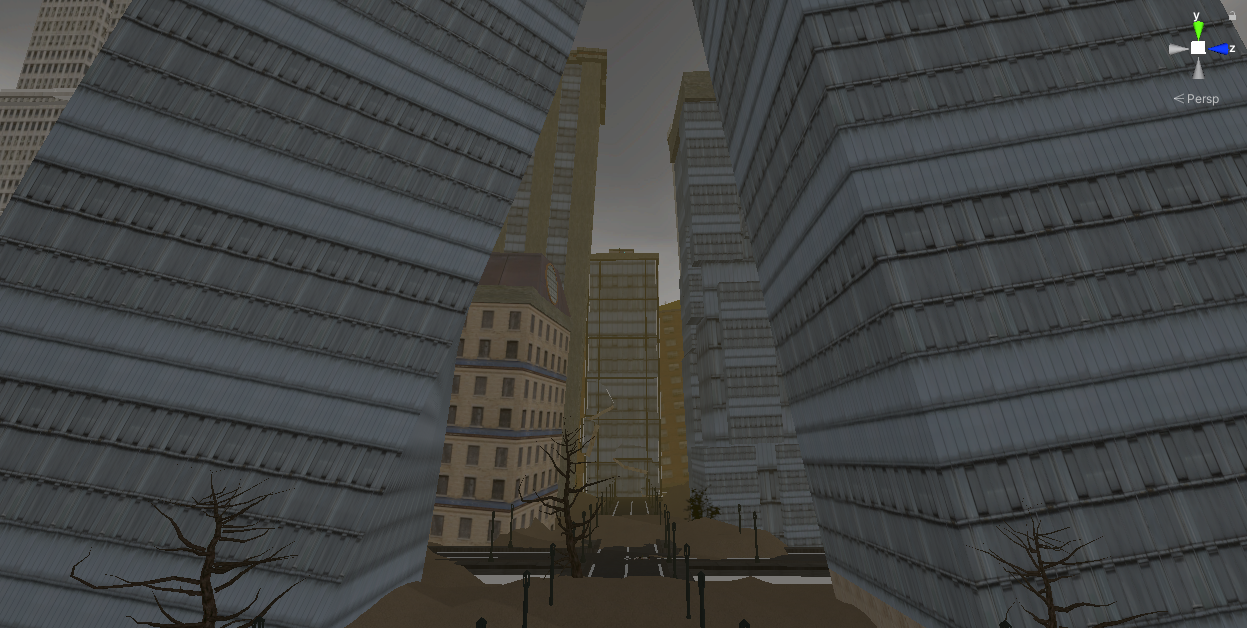
\includegraphics[scale=0.3]{pics/beamvr_yellow_fog}
    \caption{Beam VR - Yellow Fog}
    \label{fig:beamvr_yellow_fog}
\end {figure}

\subsection{Lichter}\label{subsec:light-effect}
In der Nacht Map wurden die von Unity bereitgestellten Point-Lights als Straßenlichter benutzt.
Point Lights k\"onnen mithilfe eines Radius auf einen bestimmten kreisf\"ormigen Bereich eingegrenzt werden.
Weiters wird mithilfe der Lichtst\"arke die Wirkkraft des Lichtes in diesem Gebiet genauer bestimmt.
Dank diesen Eigenschaften war das Point Light perfekt f\"ur die aufhellung der Straßen.
~\ref{fig:beamvr_street_lights}
~\cite{Unity_PointLights_2022}
\begin {figure}
    \centering
    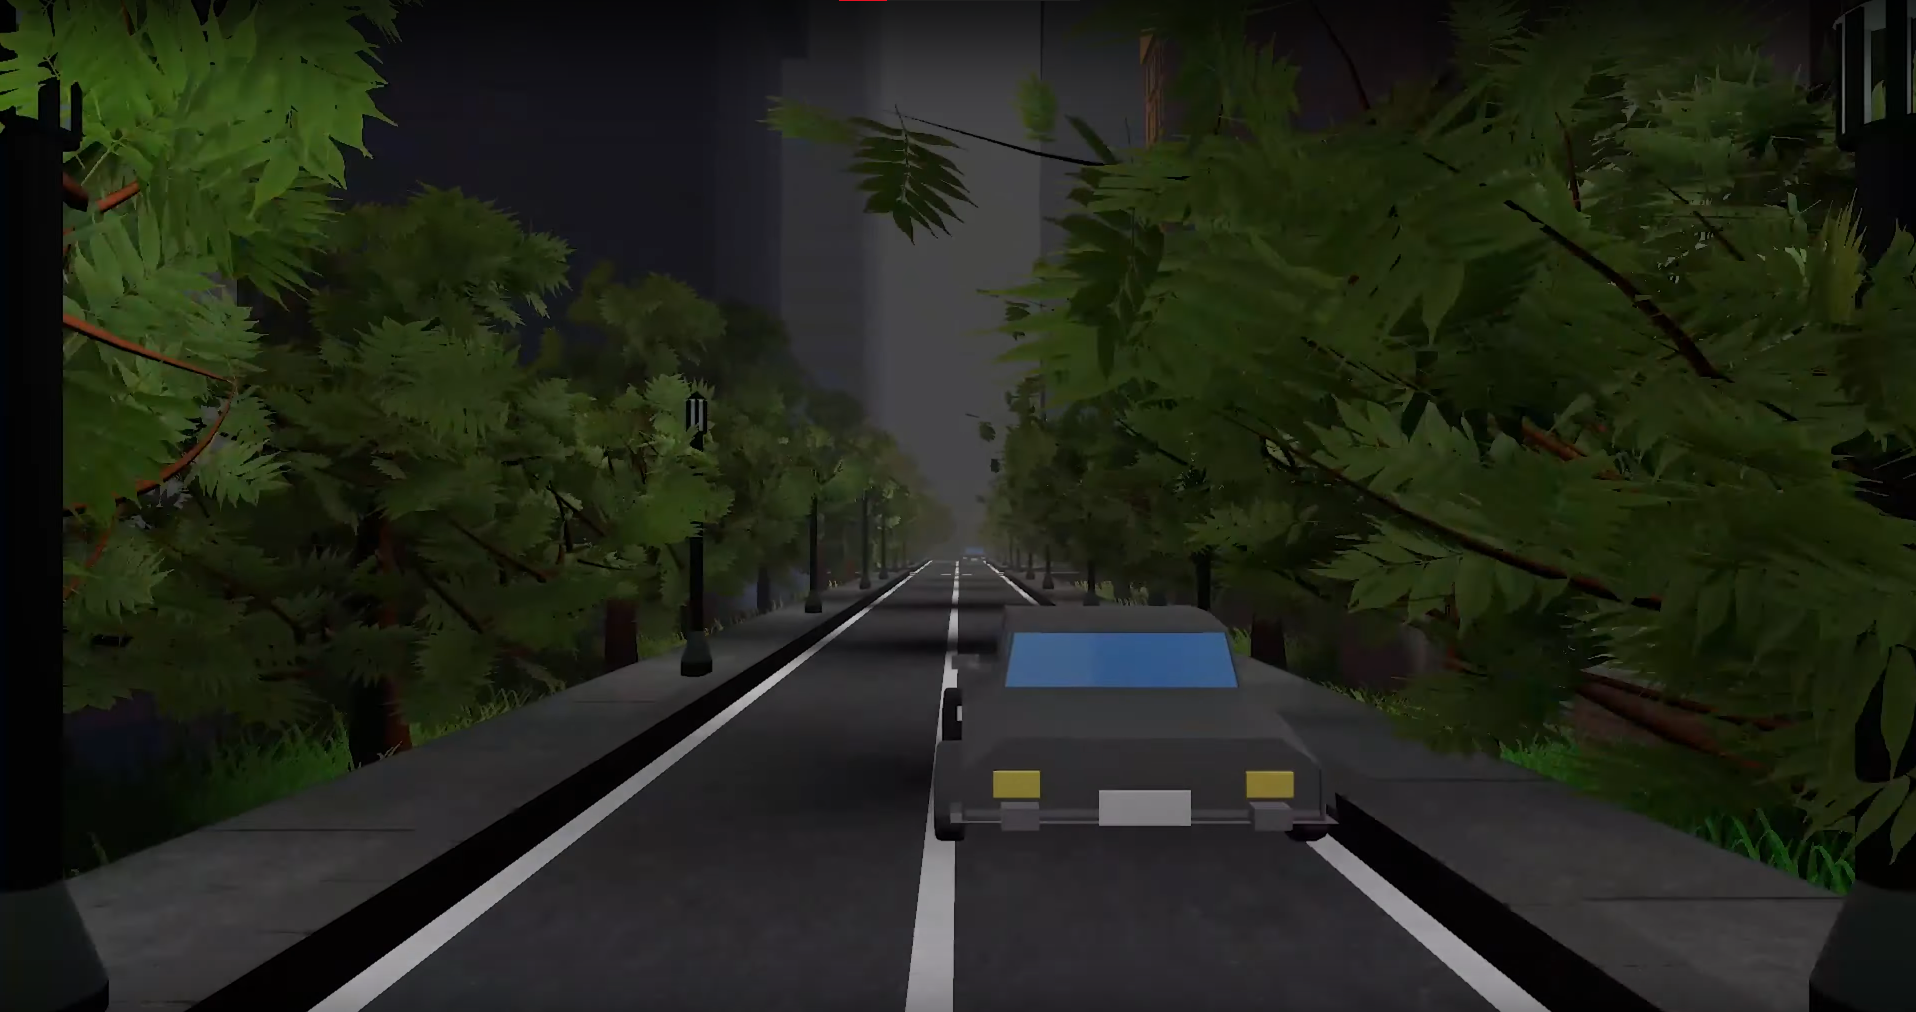
\includegraphics[scale=0.3]{pics/beamvr_point_lights}
    \caption{Beam VR - Street Lights}
    \label{fig:beamvr_street_lights}
\end {figure}


\subsection{Wind}\label{subsec:wind-effect}
Damit sich die B\"aume und B\"usche in BeamVR wie im Wind bewegen, werden Unitys Wind Zones ben\"otigt.
Diese Zonen sind bestimmte Bereiche, in welchen eine Windrichtung, Windst\"arke und Turbulenz definiert wird.
Die eingestellten Effekte werden dann auf alle Objekte angewandt, die mithilfe des Terrains oder Particle Systems iniziiert wurden.
~\cite{Unity_WindZones_2022}

\section{Unity Prefabs}\label{sec:prefabs}
\subsection{Game}\label{subsec:game-prefab}
\subsection{CameraRigGame}\label{subsec:camera-rig-game-prefab}
\subsection{CameraRigMenu}\label{subsec:camera-rig-menu-prefab}
\section{Inbetriebnahme}\label{sec:commissioning}
